\documentclass[tikz,border=10pt]{standalone}
\usepackage{tikz}
\usetikzlibrary{positioning}
\usetikzlibrary{calc}

\begin{document}
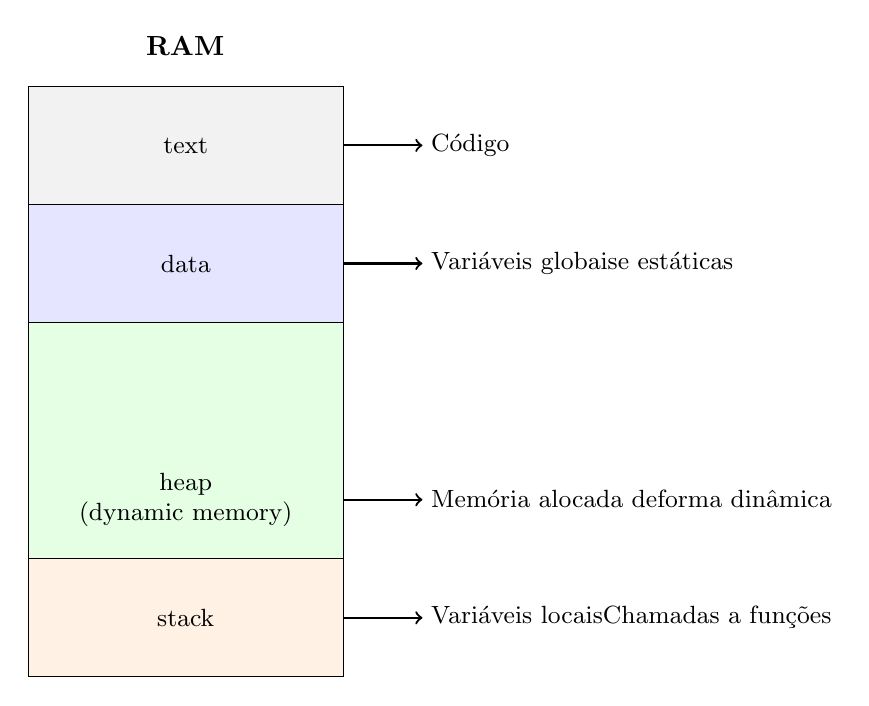
\begin{tikzpicture}[
  section/.style={draw, minimum width=4cm, minimum height=1.5cm, anchor=north west, align=left, font=\small},
  label/.style={font=\small, anchor=west},
  bigsection/.style={section, minimum height=4.5cm, anchor=north west, align=center, font=\small}
]

% RAM label
\node[font=\bfseries] at (2, 0.5) {RAM};

% Sections (top-down)
\node[section, fill=gray!10] (text) at (0, 0) {text};
\node[section, fill=blue!10] (data) at (0, -1.5) {data};
\node[bigsection, fill=green!10] (heap) at (0, -3) {heap \\ (dynamic memory)};
\node[section, fill=orange!10] (stack) at (0, -6) {stack};

% Right side descriptions
\node[label] at (5, -0.75) {Código};
\node[label] at (5, -2.25) {Variáveis globais \\ e estáticas};
\node[label] at (5, -5.25) {Memória alocada de \\ forma dinâmica};
\node[label] at (5, -6.75) {Variáveis locais \\ Chamadas a funções};

% Optional arrows (visual correspondence)
\draw[->, thick] (text.east) -- ++(1, 0);
\draw[->, thick] (data.east) -- ++(1, 0);
\draw[->, thick] (heap.east) -- ++(1, 0);
%\draw[->, thick] ($(heap.north east)!0.5!(heap.south east)$) -- ++(1, 1);

\draw[->, thick] (stack.east) -- ++(1, 0);

\end{tikzpicture}
\end{document}
